\documentclass{article}
\usepackage{enumitem}
\usepackage{graphicx}
\oddsidemargin=0in
\evensidemargin=0in
\textwidth=6.5in
\topmargin=-.5in
\textheight=9in
\parindent=0in
\pagestyle{empty}

\begin{document}
\begin{center}
  \Large\textbf{Batteries and bulbs activity}
\end{center}

Obtain a single battery, bulb, and wire. Connect them in as many ways as you can.
\begin{enumerate}
  \item  Sketch at least two arrangements that cause the bulb to light up and at least two that don't.
  \item Summarize how a battery and bulb must be connected to light the bulb.
\end{enumerate}

\begin{figure}[h]
  \centering
  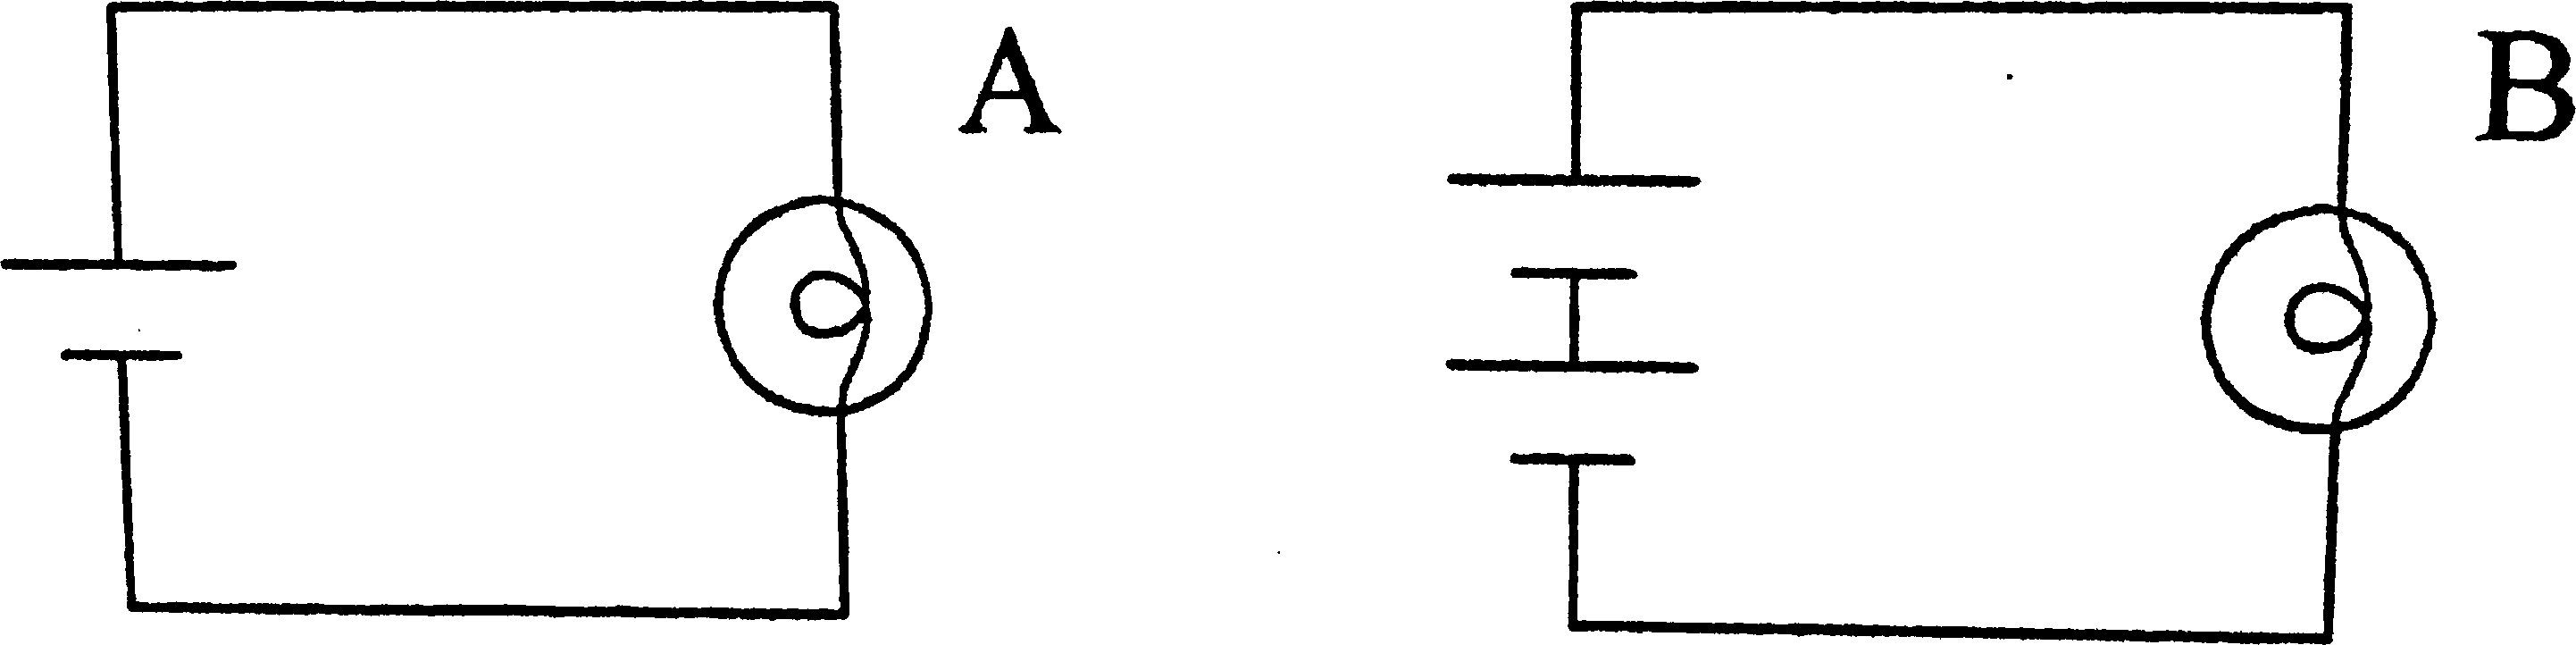
\includegraphics[width=1.5in]{1.png}
\end{figure}
\begin{enumerate}[resume]
  \item Refer to the diagram above. Predict which bulb will be brighter.
  \item Create the circuits and test your prediction. Write down the result. Was your prediction correct?
\end{enumerate}

Current is the word for whatever it is that flows through an electric circuit.
An ammeter measures current. IMPORTANT: THE AMMETER MUST \textbf{NEVER} BE CONNECTED DIRECTLY ACROSS THE BATTERY OR IT WILL BE DAMAGED. IT MUST ALWAYS BE IN SERIES WITH A ``RESISTANCE''.
\begin{figure}[h]
  \centering
  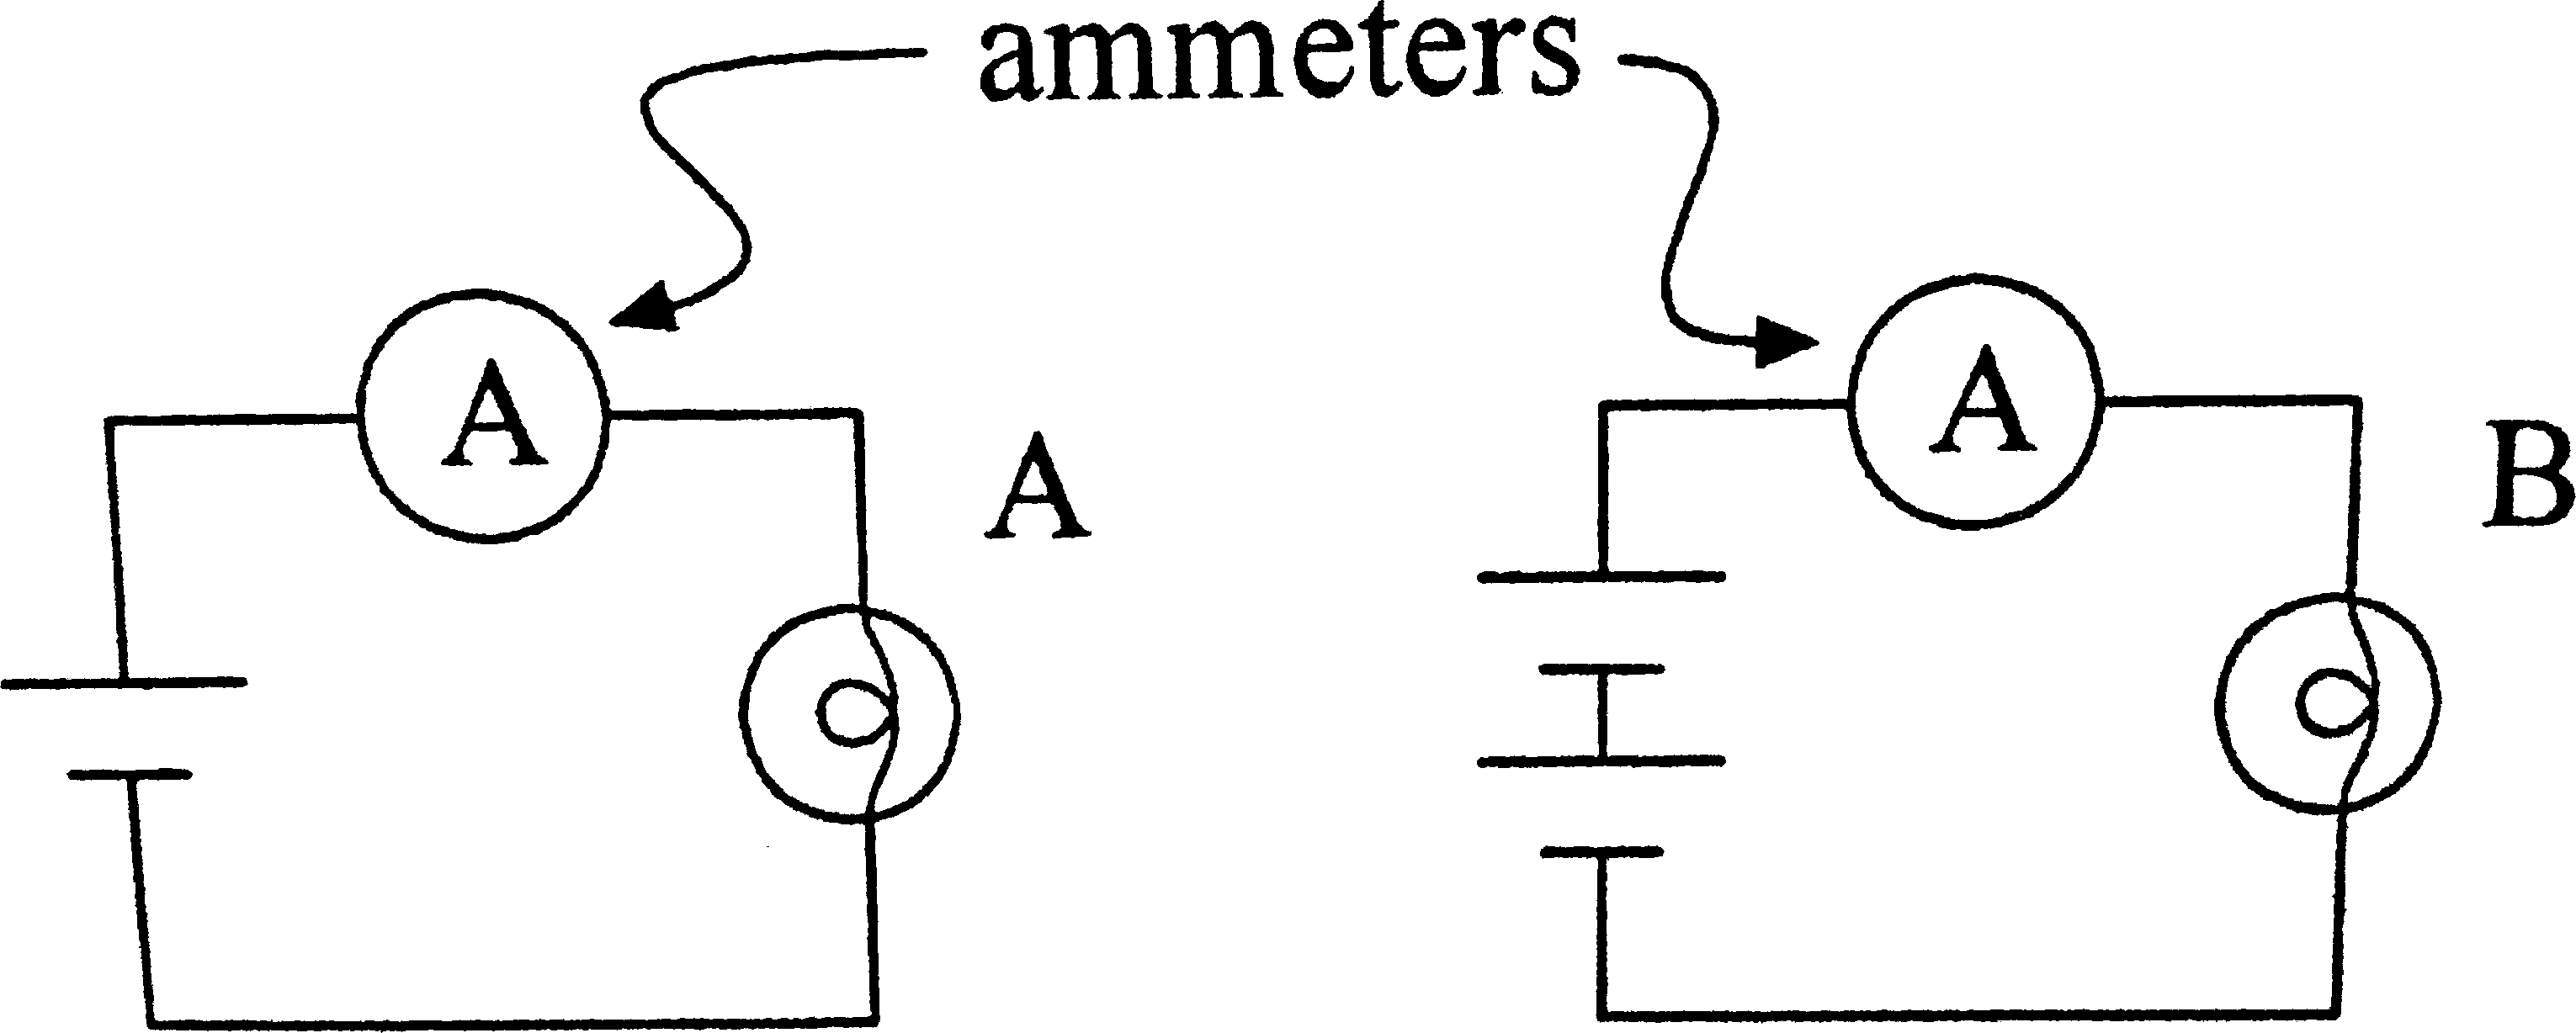
\includegraphics[width=1.5in]{2.png}
\end{figure}
Hook up an ammeter in series with each of the circuits from the previous part, as shown in the figure.
\begin{enumerate}[resume]
  \item How does the reading on the ammeter compare to the brightness of the bulb?
  \item How does a bulb indicate the current flowing through it?
  \item How does an ammeter indicate the current flowing through it?
\end{enumerate}

\begin{figure}[h]
  \centering
  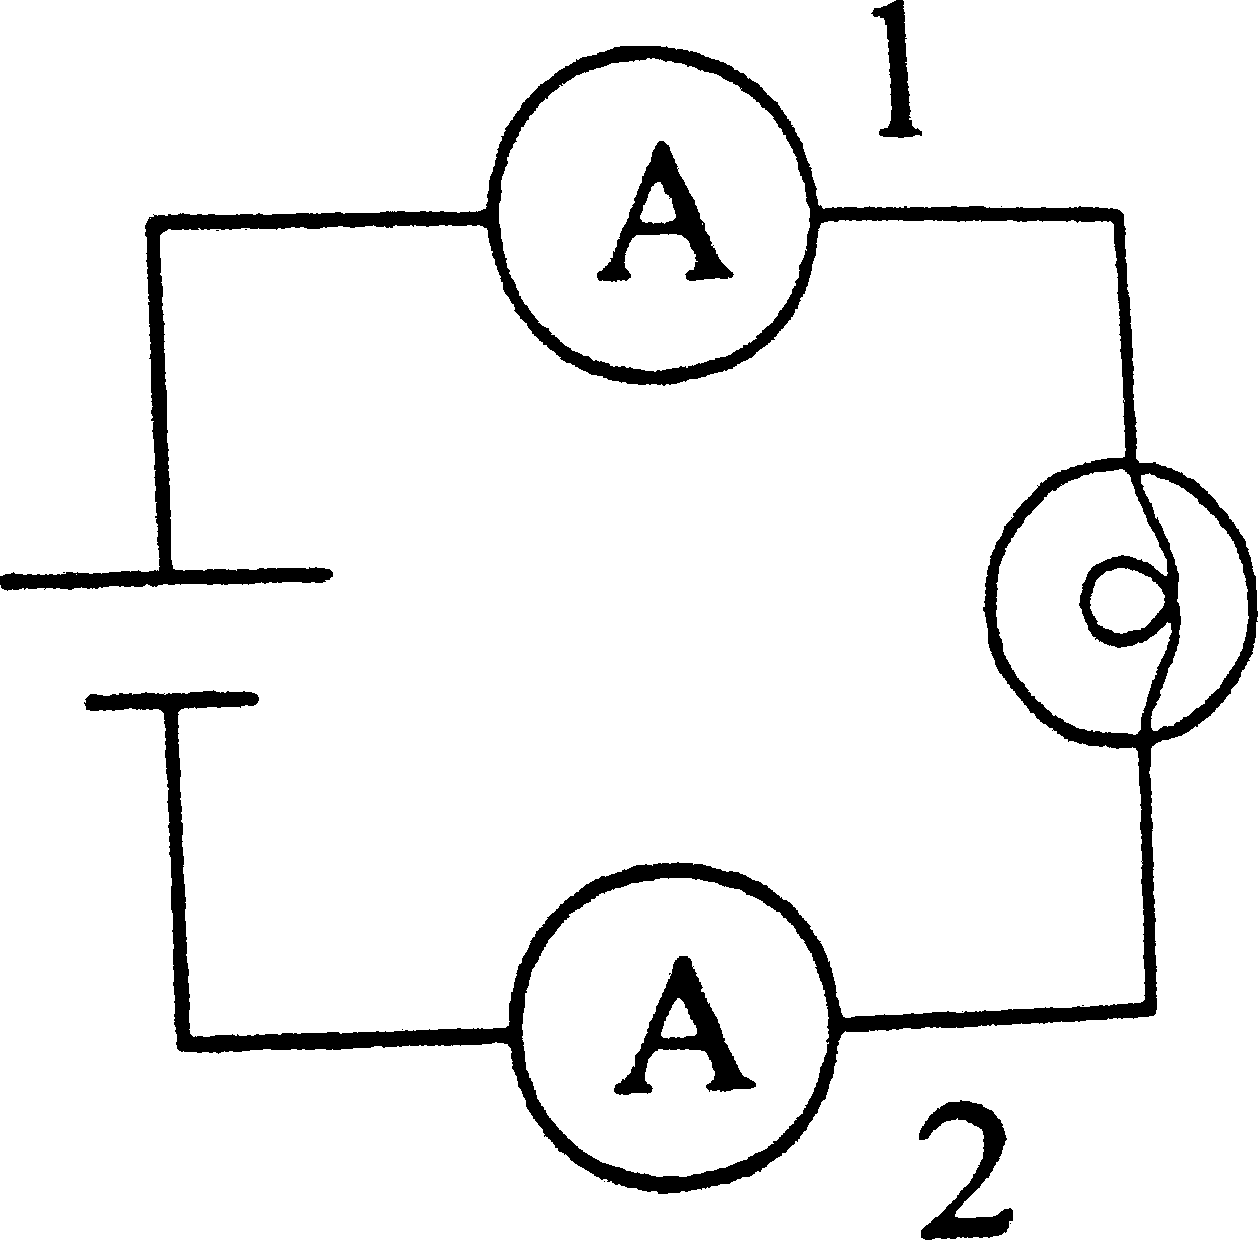
\includegraphics[width=1in]{3.png}
\end{figure}
Move the ammeter ``around'' the circuit, as shown above.
\begin{enumerate}[resume]
  \item How do the current readings at different places compare?  Be sure that you measure the current ``before'' the bulb (position 1) and ``after'' the bulb (position 2).
  \item How much of the current that enters a bulb then leaves it? 
  \item Is current ``used up'' after it passes through a bulb?
\end{enumerate}

\newpage{}

\begin{figure}[h]
  \centering
  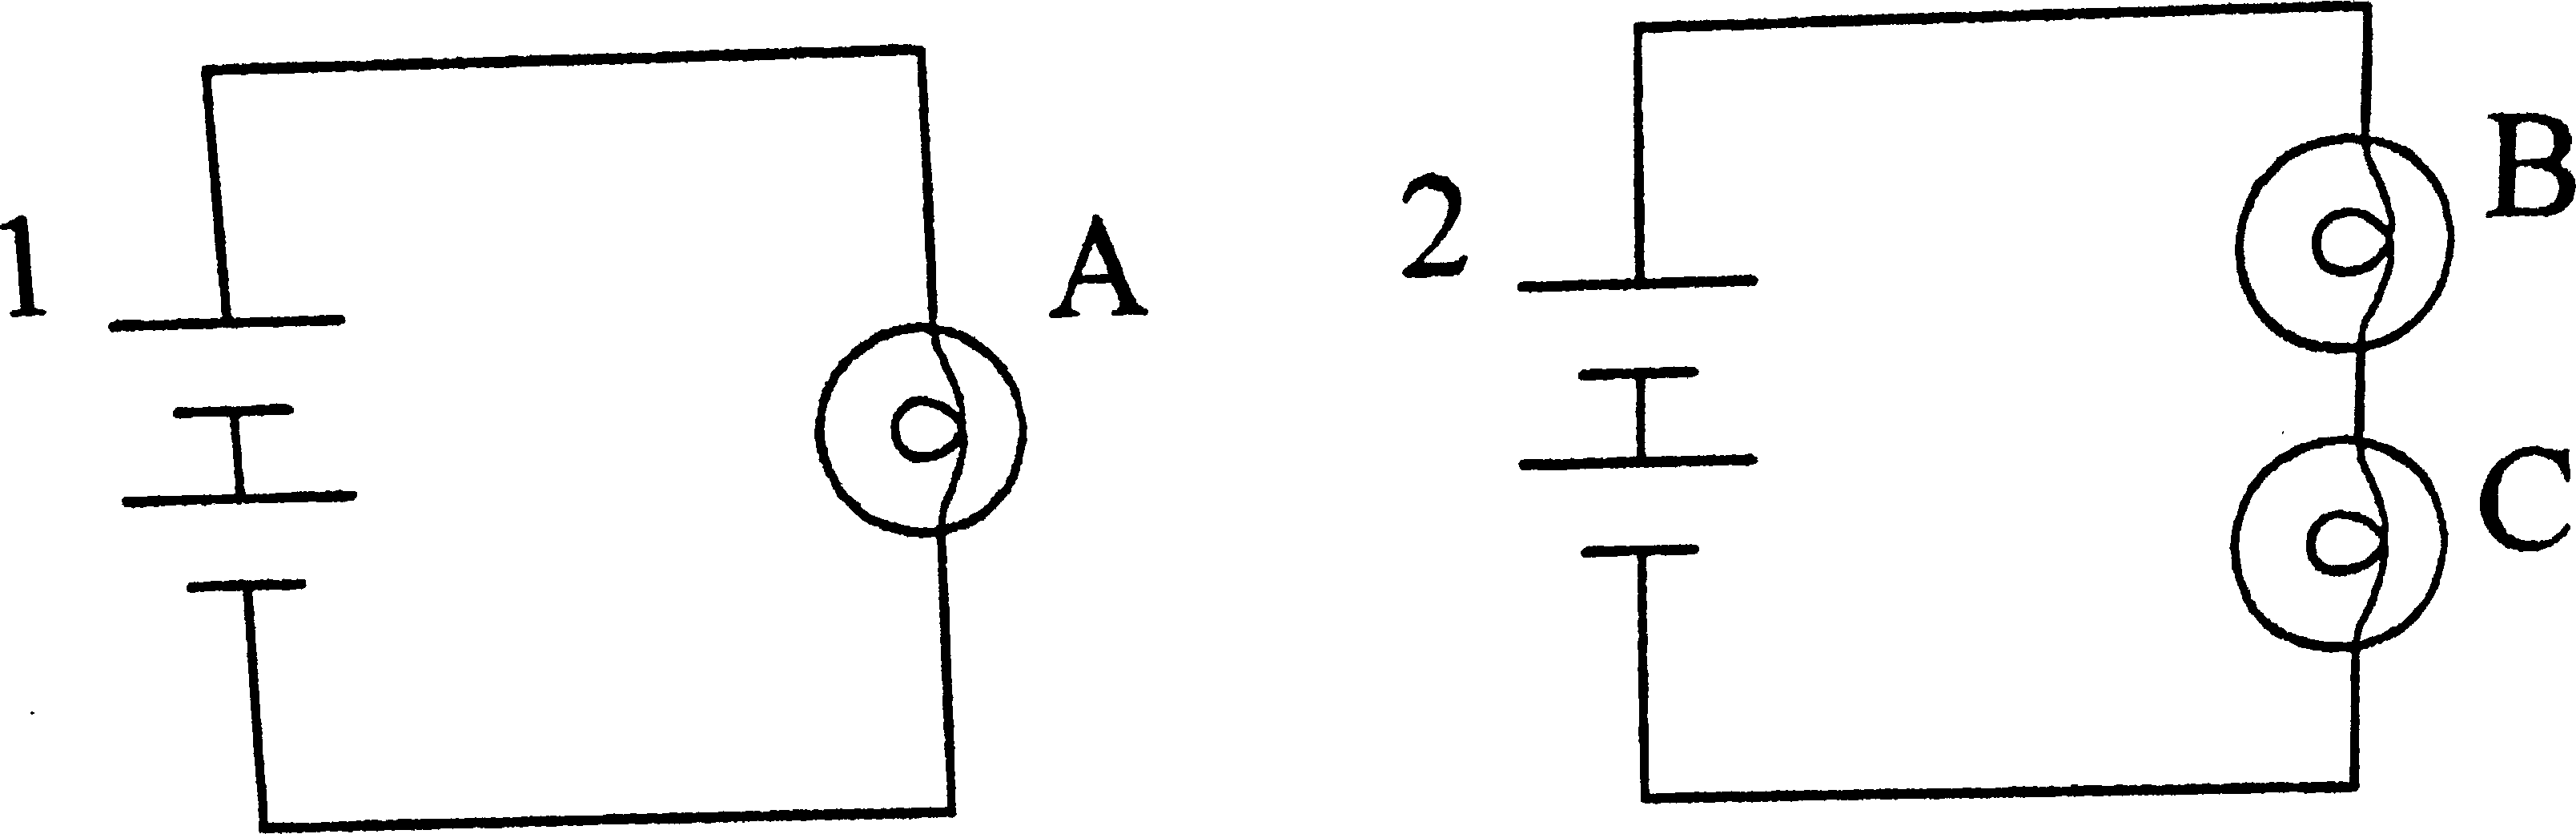
\includegraphics[width=1.5in]{4.png}
\end{figure}
\begin{enumerate}[resume]
  \item Refer to the diagram above. Predict the relationship of brightness between the three bulbs.
  \item Create the circuits and test your prediction. Write down the result. Was your prediction correct?
  \item How does current change when bulbs are added in series?
  \item A bulb can be thought of as an obstacle or resistance to current. How does the \textbf{total} resistance in a circuit change when bulbs are added in series?
\end{enumerate}
\begin{figure}[h]
  \centering
  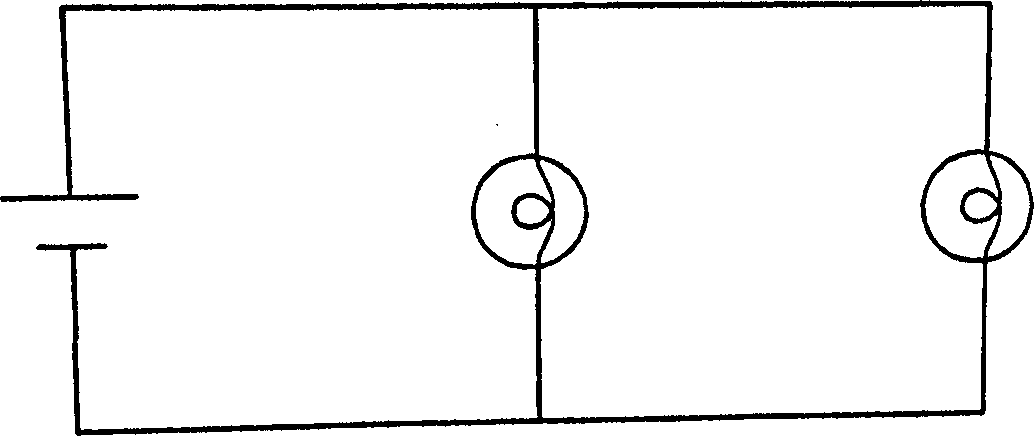
\includegraphics[width=1.5in]{5.png}
\end{figure}
\begin{enumerate}[resume]
  \item Instead of having B and C in series, the diagram above has them in parallel. Predict the relationship of brightness between A and the `new' B and C.
  \item Create the circuits and test your prediction. Write down the result. Was your prediction correct?
  \item Predict how the current through the battery in the series case compares to the parallel case.
  \item Use an ammeter to test your prediction. Write down the result. Was your prediction correct?
  \item How is the current through the battery in a parallel circuit related to the current through each bulb?
  \item How does the \textbf{total} resistance in a circuit change when bulbs are added in parallel? Compare this answer with the series case, above.
\end{enumerate}

\end{document}
